\documentclass[12pt,a4paper]{article}
\usepackage[utf8]{inputenc}
\usepackage[T1]{fontenc}
\usepackage{amsmath}
\usepackage{amssymb}
\usepackage{graphicx}
\usepackage[left=2.00cm, right=2.00cm, top=2.00cm, bottom=2.00cm]{geometry}
\usepackage{hyperref}

\usepackage{setspace}
\usepackage{siunitx}
\DeclareSIUnit\rydberg{Ry}
\usepackage{tikz}
\usepackage{paralist}
\usepackage[version=4]{mhchem}
\usepackage{booktabs}
\usepackage{rotating}
\usepackage{chngcntr}

\title{Prediction of XPS binding energies for molecules grafted on calcium surfaces}
\author{Pierre Beaujean}
\date{Version of \today}

\allowdisplaybreaks
\onehalfspacing

\def\dbe{\ensuremath{\Delta\text{BE}}}

\begin{document}
\maketitle

\section{Introduction}

Batteries are one of the key enabling technologies to transition to a climate-neutral society. Since their market introduction, lithium-ion batteries (LIB) have developed into a very mature technology and are currently used in a multitude of applications. However, while the established LIBs provide acceptable performances, these are unlikely to meet the foreseen objectives required for the large-scale applications, due to 3 key issues: \begin{inparaenum}[i)]
	\item availability of raw materials (currently involving rare-earth metals), 
	\item low energetic density, and 
	\item poor sustainability among a large number of cycles. 
\end{inparaenum}
The ECOBAT project propose to tackle the second point by using divalent cations, such as  \ce{Ca^2+} However, it is highly reactive and requires specially designed electrolytes to achieve a reversible mechanism. To do so, understanding the chemistry of its solid-electrolyte interphase (SEI) is also important. 

In the literature, calcium batteries (CIB)  use carbonate-containing electrolytes such as  dimethtyl ether (DME), ethylene carbonate (EC), glyme, or tetrahydrofuran (THF), mixed with weakly coordinated anions such as \ce{BH4-} or \ce{BF4-} \cite{zhaoRevealingSolidElectrolyte2022,taghavi-kahaghPoweringFutureComprehensive2023}.  While there exists some experimental \cite{melemedImpactDifferentialCa22023} and theoretical \cite{hahnCriticalRoleConfigurational2020,liepinyaComputationalComparisonEther2021,pathreekerWhyTetrahydrofuranGood2021,yamijalaStabilityCalciumIon2021} studies on the SEI  formation, we would like provide a better understanding by means of spectroscopic tools, by combining experimental spectra with theoretical calculations.

X-ray photoelectron spectroscopy (XPS) is a surface sensitive quantitative spectroscopy, which allows performing identification of elements within the material or at its surface. It belongs to the family of photoemission spectroscopies, where the energy of electrons emitted by means of the photoelectric effect is analyzed. In particular with XPS, a beam of soft X-rays (\SI{100}{\electronvolt} < $h\nu$ < \SI{10}{\kilo\electronvolt}) are used, so that core electrons (low principal quantum number) may be probed \cite{stevieIntroductionXrayPhotoelectron2020}.  It is therefore routinely used to gain understanding in SEI composition, both experimentally \cite{melemedImpactDifferentialCa22023} and theoretically \cite{ebadiInsightsLiMetalOrganic2019}.

In this study, we focus on the XPS spectra from the degradation of THF as a toy model. To do so, different possible degradation products (Fig.~\ref{fig:THFdegradation}) will be considered on different possible calcium substrate, including calcium oxide and hydride.

\begin{figure}
	\centering
	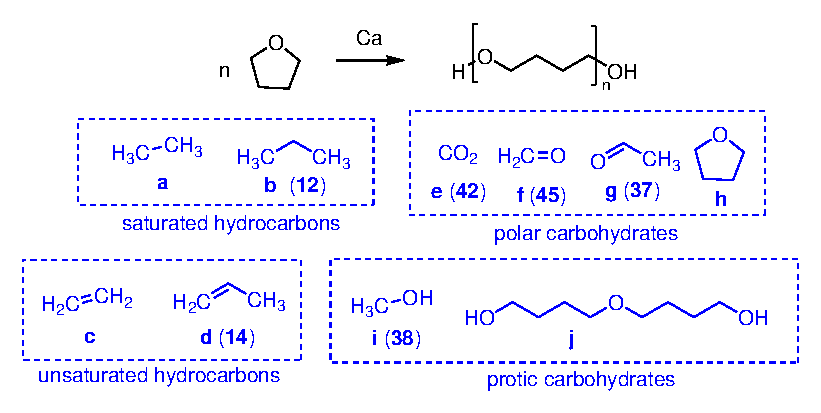
\includegraphics{Figure1}
	\caption{The main degradation pathway of THF leads to THF polymer (black). Compound \textbf{a}-\textbf{i} (blue) are considered in this study: \textbf{a} is used as a model for the THF polymer, while fragmentation may lead to (un)saturated hydrocarbons (\textbf{b}-\textbf{e}) or carbonates (\textbf{f}-\textbf{i}).}
	\label{fig:THFdegradation}
\end{figure}

\section{Theoretical methods}

In XPS spectroscopy, conservation of energy dictates :\begin{equation}
	h\nu =\text{BE} + E_{kin} + \phi, \label{eq:xps}
\end{equation}
where BE  is the binding energy (BE) of the electron, $E_{kin}$ is the kinetic energy of the emitted electron (measured by the detector) and $\phi$ is the work function, which appears in the case of a surface (and, in practice, is also due in part to the detector). Using a source of monochromatic X-rays (such as Al $K_\alpha$, $h\nu = \SI{1486.7}{\electronvolt}$), it is possible to determine BE, the quantity of interest, from $E_{kin}$ \cite{vinesPredictionCoreLevel2018}.
This binding energy depends on how tight the electron is bound to its orbital. It is therefore sensitive to the oxidation state and \textit{chemical environment} of its origin atom (roughly speaking, the more electronegative are the surrounding atoms, the largest BE). Thus, much like the chemical shifts in NMR, this technique provides information on the surroundings of a given atom. 
From a quantum chemistry point of view, a binding energy is nothing much than an ionization energy of the core electrons:\begin{equation}
	\text{BE}_i = E^{N-1}_i(\text{final}) - E^{N}(\text{initial}), \label{eq:dscf}
\end{equation}
where $E^{N}$ and $E^{N-1}$ are the energies of the initial $N$-electron non-ionized and the final $N-1$ electrons ionized state, which contains a so-called core hole on atom $i$. While these energies could be obtained through (relativistic) multi-configuration approaches, it is impractical for large systems. Even CIS (or TD) excitations are difficult to target, since they generally correspond to highly excited roots  \cite{vinesPredictionCoreLevel2018}.

For molecules in the gas phase, ``classical'' quantum chemistry tools can be used. At the HF level of theory, core level BE might be approached by means of Koopmans' theorem, \textit{i.e.}, the energy of the orbital from which the electron is removed. This approach is also referred to as the initial state (IS) of frozen orbitals (FO) approach (\textit{vide supra}). However, relaxation effects are neglected. More accurate values can be obtained by means of Eq.~\eqref{eq:dscf}, by computing the energy difference between initial and finale states at the HF level, which is generally referred to as the $\Delta$SCF approach in the literature, and include the so-called final state (FS) effects.	Though it might provide quantitative agreement in some case, electron correlation effect can be important and density functional theory (DFT) should be used, for which Koopman's theorem no longer holds \cite{pueyobellafontPredictingCoreLevel2017}.

Things are even more difficult when solids or surfaces are treated. Generally, to avoid the huge computational costs, only valence levels are explicitly treated, while pseudopotentials (PPs) model the core electrons. Then, the projected augmented wave method (PAW) provides a way to map the results to all-electron wave function by resorting to specially designed PPs and a set of transformations \cite{blochlProjectorAugmentedwaveMethod1994}. In some code, such as CP2K or VASP, it is possible to generate a core hole, which will neglect the relaxation of the (other) core electrons but will include the one of the valence electrons. This prevents an accurate description of absolute BE.

An additional problem is that when using periodic boundary conditions, the core hole is periodically repeated, resulting in a infinitely charged system. To circumvent this problem two approaches might be used: \begin{inparaenum}[a)]
	\item the excited electron is added to the bottom of the (former) conduction band (or LUMO, for isolated molecules), or
	\item the excited electron is removed from the system and a background of (counter-)charge is used.
\end{inparaenum}
It is obvious that while the first approach is actually similar to an absorption process (and will underestimate the BEs), the second also induces physically incorrect effects. This further prevents the prediction of absolute BE.
It is however possible to estimate (relative) BE, by computing wave function for a fractional number of electron, thanks to the so-called Slater transition state theory wich with the help of the Janak theorem \cite{janakProofThatFrac1978}, results in the Slater-Janak (SJ) approach \cite{hiraoImprovedSlaterTransition2021}. In the following, BE are computed with a half-electron, put either in the conduction band or in the vacuum, referred to as the SJ and SJ\textsuperscript{n} approaches, respectively (Fig.~\ref{fig:method}).
	
	\begin{figure}[!h]
		\centering
		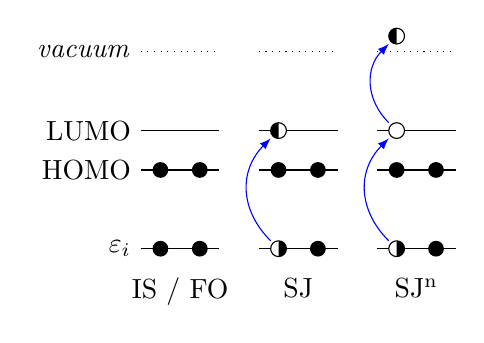
\begin{tikzpicture}
			\draw (0,0) node[left]{$\varepsilon_i$}-- node[midway,below=.25cm]{IS / FO} +(1,0);
			\draw (0,1) node[left]{HOMO}-- +(1,0);
			\draw (0,1.5) node[left]{LUMO}-- +(1,0);
			\draw[dotted] (0,2.5) node[left]{\textit{vacuum}}-- +(1,0);
			\fill (.25,0) circle (.1cm);
			\fill (.75,0) circle (.1cm);
			\fill (.25,1) circle (.1cm);
			\fill (.75,1) circle (.1cm);
			
			\begin{scope}[xshift=1.5cm]
				\draw (0,0) -- node[midway,below=.25cm]{SJ} +(1,0);
				\draw (0,1) -- +(1,0);
				\draw (0,1.5) -- +(1,0);
				\draw[dotted] (0,2.5) -- +(1,0);
				\draw[fill=white] (.25,0) circle (.1cm);
				\fill (.25,-.1) arc (-90:90:.1);
				\fill (.75,0) circle (.1cm);
				\fill (.25,1) circle (.1cm);
				\fill (.75,1) circle (.1cm);
				\draw[fill=white] (.25,1.5) circle (.1cm);
				\fill (.25,1.4) arc (-90:-270:.1);
				\draw[-latex,blue] (.15,.1) .. controls +(-.4,.4) and +(-.4,-.4) .. (.15,1.4);
			\end{scope}
			
			\begin{scope}[xshift=3cm]
				\draw (0,0) -- node[midway,below=.25cm]{SJ\textsuperscript{n}} +(1,0);
				\draw (0,1) -- +(1,0);
				\draw (0,1.5) -- +(1,0);
				\draw[dotted] (0,2.5) -- +(1,0);
				\draw[fill=white] (.25,0) circle (.1cm);
				\fill (.25,-.1) arc (-90:90:.1);
				\fill (.75,0) circle (.1cm);
				\fill (.25,1) circle (.1cm);
				\fill (.75,1) circle (.1cm);
				\draw[fill=white] (.25,1.5) circle (.1cm);
				\draw[-latex,blue] (.15,.1) .. controls +(-.4,.4) and +(-.4,-.4) .. (.15,1.4);
				\draw[-latex,blue] (.15,1.6) .. controls +(-.3,.3) and +(-.3,-.3) .. (.15,2.6);
				\draw[fill=white] (.25,2.7) circle (.1cm);
				\fill (.25,2.6) arc (-90:-270:.1);
			\end{scope}
		\end{tikzpicture}
		\caption{Approaches to compute BE as the energy of the molecular orbital where the core hole is located: initial state (IS, also referred to as frozen orbitals, FO) and Slater-Janak (SJ). When the electron is further removed from the system (and conceptually pushed to the vacuum), JS\textsuperscript{n} is noted. Adapted from Ref.~\cite{pueyobellafontPredictingCoreLevel2017}.}
		\label{fig:method}
	\end{figure}

Finally, while the determination of absolute BE is difficult from a theoretical point of view, the measurement (or the calculation) of the work function, $\phi$  in Eq.~\eqref{eq:xps}, is not simple either, so both experimentalist and quantum chemists actually focus on \dbe{}, the difference of binding energy for a given atom with respect to a reference compound \cite{vinesPredictionCoreLevel2018}. Therefore, relative BE computed as $\dbe_i =\text{BE}_i-\text{BE}(\text{ref})$, are reported in this contribution, using the calculated/experimental BE values for \ce{CH4}, \ce{NH3}, \ce{H2O}, \ce{BH2BH2}, and \ce{HF} as references for carbon, nitrogen, oxygen, boron, and fluorine, respectively (experimental values are from Ref.~\cite{pueyobellafontPredictingCoreLevel2017}). 
	
\section{Computational details}

Unless otherwise mentioned, all calculations were performed at the PBE-D3 level using VASP (version 6.4.1) with the projector-augmented wave (PAW) method \cite{blochlProjectorAugmentedwaveMethod1994}.  Convergence of the energy is set to \SI{e-4}{\electronvolt} with a cutoff of \SI{550}{\electronvolt} for the kinetic energy of the plane-waves. Gaussian smearing of the valence electrons, with a width of \SI{0.2}{\electronvolt}, is used. The Brillouin zone integration integration for molecule in gas phase, bulk, and slabs were performed at gamma point, and using a 4x4x4 and 4x4x1 Monkhorst and Pack k-point mesh, respectively. The \texttt{Ca\_sv} pseudopotential was used to model calcium.

All optimizations are carried on using the L-BFGS algorithm, driven by ASE \cite{larsenAtomicSimulationEnvironment2017} using the VASP energies and forces, until the force on all atom is lower than \SI{e-2}{\electronvolt\per\angstrom}.\footnote{Pour faire de la spectroscopie IR, le but sera d'arriver par la suite à \SI{e-3}{\electronvolt\per\angstrom}, ou bien on a des grosses (>\SI{1000}{\per\centi\meter}) fréquences imaginaires!}

For the calculation of BE, VASP allow to target a specific orbital, $i$, from which the half electron is removed. For SJ\textsuperscript{n}, it is also mandatory to set the appropriate number of valence electrons (with the \texttt{NELECT} keyword). After the calculation, its eigenvalue, $\varepsilon_i\left(\frac{1}{2}\right)$, is extracted. Then,
\begin{equation}
	\text{BE}_i = 	\begin{cases}
		-\varepsilon_i\left(\tfrac{1}{2}\right) & \text{if  gas phase}, \\
	E_F-\varepsilon_i\left(\tfrac{1}{2}\right) & \text{otherwise}. \label{eq:xpsbe}
	\end{cases}
\end{equation}
where,  to be consistent from one system to another, results for slabs are shifted by the Fermi energy, $E_F$ (computed while setting \texttt{EFERMI = MIDGAP} in the VASP input to account for Gaussian smearing). However doing this correction in gas phase results in inconsistent results, as demonstrated in Figure \ref{fig:xps_C185_fermi}. It also gives incoherent results when used on bulks, as the Fermi level is not well defined by VASP in such case.


\paragraph{Binding energies of molecules in gas phase.} In order to assess the quality of the SJ and SJ\textsuperscript{n} approaches, the results from  Belafont \textit{et al}. \cite{pueyobellafontPredictingCoreLevel2017}, which compare experimental and theoretical calculations of gas phase \dbe, is replicated. To do so, their set of 184 experimental absolute BE (Fig.~\ref{fig:core185}) coming from 68 molecules and spanning carbon (N=107), nitrogen (N=20), oxygen (N=22), boron (N=20), and fluorine (N=15) atoms is used. After an optimization, each molecule is placed in a cubic box of \SI{20}{\angstrom} of side, and BE are computed for each atom of interest.

\begin{figure}[!h]
	\centering
	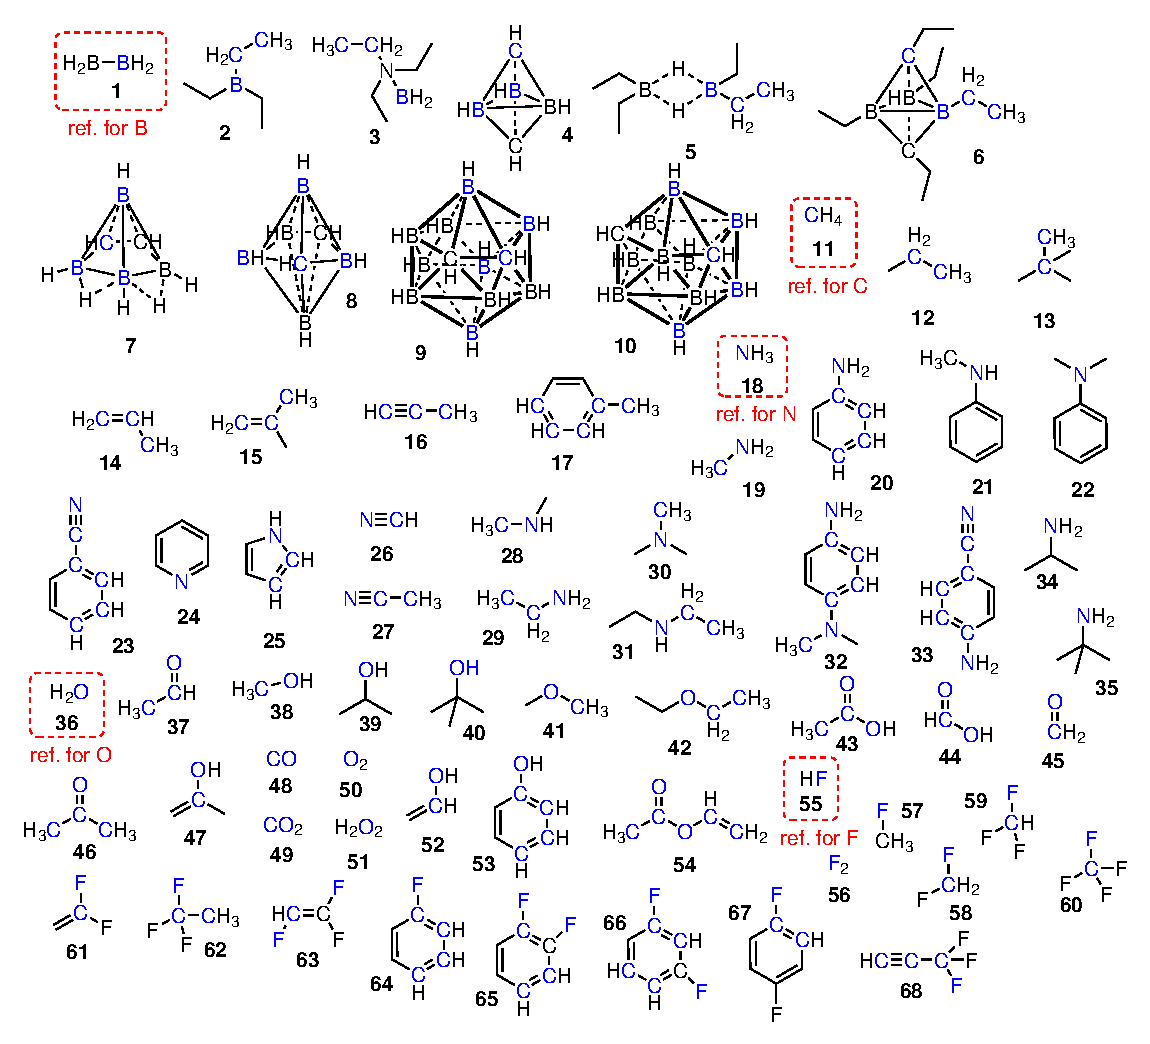
\includegraphics[width=\linewidth]{Figure3}
	\caption{Molecules for the benchmark \cite{pueyobellafontPredictingCoreLevel2017}. The atoms for which experimental BE are provided are highlighted in blue.  The reference compound used for each atom are highlighted in red.}
	\label{fig:core185}
\end{figure}

\paragraph{Binding energies of molecules grafted on surfaces.} Following the protocol established by Ebadi and co-workers \cite{ebadiInsightsLiMetalOrganic2019}, \dbe{} of molecules adsorbed on surface were studied. First, bulk Ca (from the Material Project, \texttt{MP-45}), CaO (\texttt{MP-2605}), and \ce{CaH2} (\texttt{MP-23713}) are selected and their atomic positions and cell parameters optimized.

Then, in order to select the surface orientation, 1x1 slabs with increasing thickness along different low index surface orientation [(100), (110), and (111)], are created using ASE \cite{larsenAtomicSimulationEnvironment2017} (with a distance between two slab repetition equals to 10 times the $c$ cell parameters of the bulk) and their geometries relaxed (keeping the cell and two layers in the middle frozen, in order to mimic the impact of the bulk). For each orientation, the surface energy $\gamma^{hkl}$, was determined via a least-square fit of the following expression \cite{sunEfficientCreationConvergence2013,tranSurfaceEnergiesElemental2016}:\begin{equation}
E^{hkl}(N) = E_0\,N +	2A\,\gamma^{hkl} \label{eq:surf}
\end{equation}
where $N$ is the number of layers in the slab,  $A$ the slab surface, $E^{hkl}(N)$ is the energy of the (relaxed) slab cut along $(hkl)$, and $E_0$ is (approximately) the energy of the bulk. The results (Tab.~\ref{tab:surf}, Fig.~\ref{fig:surf}) demonstrate that (100) surfaces are the most favorable ones, in agreement with literature \cite{deleeuwDensityFunctionalTheory2000,ebadiInsightsLiMetalOrganic2019}.

\begin{table}[!h]
	\centering
	\begin{tabular}{lccc}
		\toprule
		&	\ce{Ca} & \ce{CaO} &	\ce{CaH2} \\
		\midrule
		(100) & 0.555 ($N\in[6,16]$) & 0.470 ($N\in[6,16]$) & 0.871  ($N\in[12,32]$)\\
		(110) & 0.630  ($N\in[6,16]$)& 1.777  ($N\in[6,16]$)& 1.109 ($N\in[12,32]$)\\
		(111) & 0.563  ($N\in[6,16]$) & 4.080  ($N\in[5,15]$)  & 1.117   ($N\in[12,32]$) \\ 
		\bottomrule
	\end{tabular}
	\caption{Surface energies ($\gamma^{hkl}$, in \si{\joule\per\meter\squared}) of Ca, CaO, and \ce{CaH2} slabs along different orientations, as determined through Eq.~\eqref{eq:surf} using the $N$ values given in parentheses.}
	\label{tab:surf}
\end{table}

Using the (100) orientation, 3x3 slabs (with 6 layers, and a vacuum of \SI{20}{\angstrom} between two slab repetition) where created and relaxed (cell parameters are kept frozen).  Since it is favorable \cite{deleeuwDensityFunctionalTheory2000}, the absorption of water on CaO surface was also considered, and an additional slab with full coverage (1 water molecule per surface Ca), referred to as \ce{CaO.H_2O}, was also optimized. Compound \textbf{a}-\textbf{i} (Fig.~\ref{fig:THFdegradation}) are then added on both side of the slab (at about $\sim\SI{5}{\angstrom}$, initially), and a final optimization was performed (cell parameters are kept frozen). Finally, BE are computed for each atom of interest.

\section{Results}

\subsection{Biding energies in gas phase}

A comparison between experimental and computed \dbe is given in Fig. ~\ref{fig:xps_C185}. On the one hand, the agreement with previous investigations \cite{pueyobellafontPredictingCoreLevel2017,golzeAccurateAbsoluteRelative2020}, the SJ\textsuperscript{n} protocol provide reliable results for all atoms, with very small mean error (<\SI{0.1}{\electronvolt}) and acceptable standard deviations (0.1 to \SI{0.4}{\electronvolt}).  It should be however noted that a reference per atom is necessary (Tab.~\ref{tab:xpssjn}), since the difference between the experimental and computed absolute BE increase with the atomic number.
On the other hand, the error with the SJ protocol is not systematic, as indicated by the large standard deviations (>\SI{0.7}{\electronvolt}). 

\begin{figure}[!h]
	\centering
	 \includegraphics[width=.8\linewidth]{Figure4}
	 \caption{Comparision between experimental and calculated gas phase \dbe{}, as computed with the SJ (blue) and SJ\textsubscript{n} (orange) protocols on the different atoms. For each of them, the error (as mean $\pm$ standard deviation) for both protocols is given.}
	 \label{fig:xps_C185}
\end{figure}

\begin{table}[!h]
	\centering
	\begin{tabular}{lcccc}
		\toprule
		& Reference & BE (exp.)  & BE (SJ\textsuperscript{n})  & $\Delta$(SJ\textsuperscript{n}- exp.)\\
		\midrule
		B1s & \ce{(BH2)2} & 196.50 & 201.47 & 4.97\\
		C1s & \ce{CH4} & 290.90 & 297.04 & 6.14\\
		N1s & \ce{NH3} & 405.60 & 413.58 & 7.98\\
		O1s & \ce{H2O} & 539.70 & 548.79 & 9.09\\
		F1s & \ce{HF} & 694.23 & 704.78 &10.55\\
		\bottomrule
	\end{tabular}
	\caption{Comparison between experimental (from Ref.~\cite{pueyobellafontPredictingCoreLevel2017}) and calculated (as computed with the SJ\textsuperscript{n} protocol) absolute BE.}
	\label{tab:xpssjn}
\end{table}

\clearpage
\subsection{Binding energies of slabs}

The impact of slab thickness on the resulting spectra is first assessed in Fig.~\ref{fig:slabsthickness}.


\begin{figure}[!h]
	\centering
	\includegraphics[width=\linewidth]{Figure5}
	\caption{Impact of the slab thickness .}
	\label{fig:slabsthickness}
\end{figure}

\clearpage
\bibliographystyle{unsrt}
\bibliography{biblio}

\clearpage
\appendix
\counterwithin{figure}{section}
\section{Appendix}
\begin{figure}[!h]
	\includegraphics[width=\linewidth]{FigureA1}
	\caption{Evolution of the surface energy for slabs of Ca, CaO, and \ce{CaH2} with increasing thickness ($N$) , as estimated by least-square fit of Eq.~\eqref{eq:surf}. For CaO, the surface energies of (110) and (111) are larger than \SI{1.25}{\joule\per\meter\squared}.}
	\label{fig:surf}
\end{figure}

\begin{figure}[!h]
	\centering
	\includegraphics[width=.8\linewidth]{FigureA2}
	\caption{Comparison between experimental and calculated gas phase \dbe{}, as computed with the SJ (blue) and SJ\textsubscript{n} (orange) protocols on the different atoms, and by shifting the BE by $E_F$ in Eq.~\eqref{eq:xpsbe}. For each of them, the error (as mean $\pm$ standard deviation) for both protocols is given.}
	\label{fig:xps_C185_fermi}
\end{figure}
	
\end{document}